\documentclass[12pt, a4paper] {ncc}
\usepackage[utf8] {inputenc}
\usepackage[T2A]{fontenc}
\usepackage[english, russian] {babel}
\usepackage[usenames,dvipsnames]{xcolor}
\usepackage{listings,a4wide,longtable,amsmath,amsfonts,graphicx}
\usepackage{indentfirst}
\usepackage{bytefield}
\usepackage{multirow}
\usepackage{float}
\usepackage{caption}
\usepackage{subcaption}
\captionsetup{compatibility=false}
\usepackage{tabularx}

\usepackage[left=2cm,right=2cm,top=2cm,bottom=2cm,bindingoffset=0cm]{geometry}

\begin{document}
\setcounter{figure}{0}
\frenchspacing
\pagestyle{empty}
\begin{center}
                            Университет ИТМО    \\
                        Кафедра вычислительной техники

\vspace{\stretch{2}}
			Основы теории автоматического управления
\end{center}
\vspace{\stretch{2}}
\begin{center}
			Лабораторная работа № 4 \\
<<Типовые динамические звенья>>
\end{center}
\vspace{\stretch{3}}
\begin{flushright}
                                    Студент:\\
                                    {\it Куклина М.Д., P3401}\\
                                    Преподаватель: \\
                                    {\it Кремлёв А.С.}
\end{flushright}
\vspace{\stretch{4}}
\begin{center}
                             Санкт-Петербург, 2018
\end{center}
\newpage

\section{Переходные характеристики исследуемых элементарных звеньев, их передаточные функции и параметры}

    \subsection{Блок 1}
		На рисунке~\ref{fig:p1} представлен график звена. По его форме можно определить,
		что это апериодическое звено второго порядка.

		При $T_1 = 4, T_2 = 1$ получаем $T_3 = 3.732, T_4 = 0.268$. Тогда
		передаточная функция принемает вид:
		\[ W(s) = \dfrac {1} {(3.732 s + 1) \cdot (0.268 s + 1)}\]

		Оба графика на рисуке~\ref{fig:pb1}.

    	\begin{figure}[ht!]
    		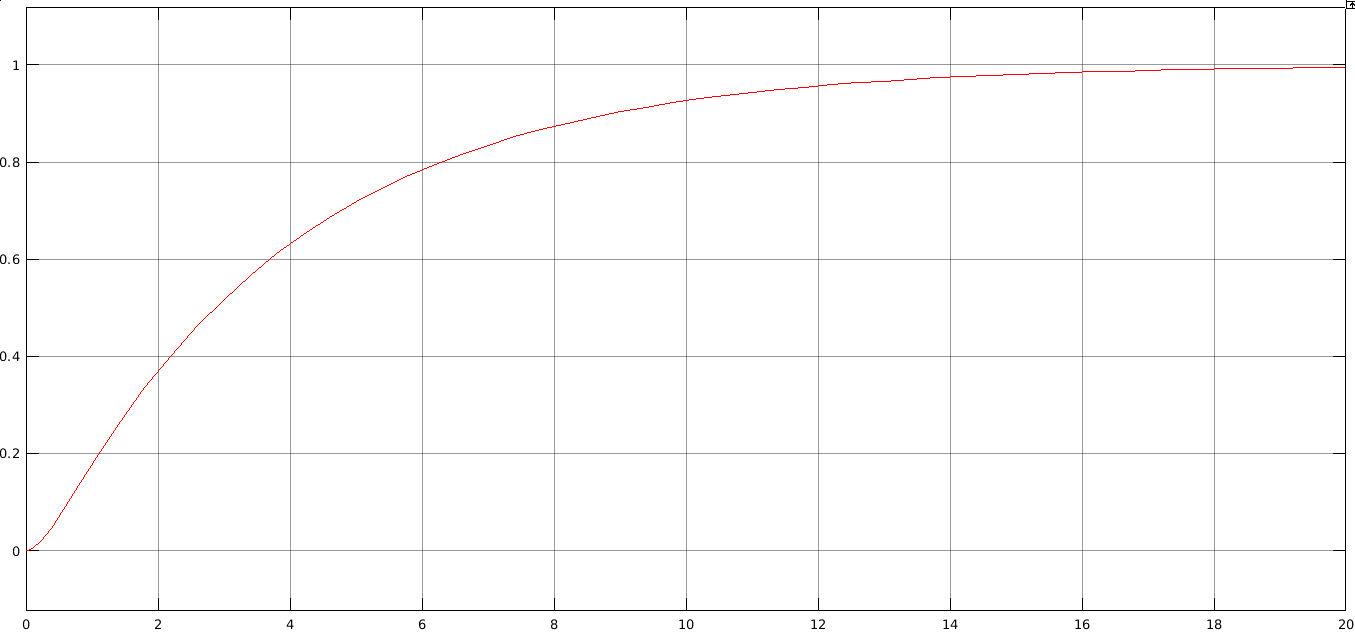
\includegraphics[scale=0.3]{./plot1.png}
			\caption{График звена в блоке 1}
			\label{fig:p1}
    	\end{figure}

    	\begin{figure}[ht!]
    		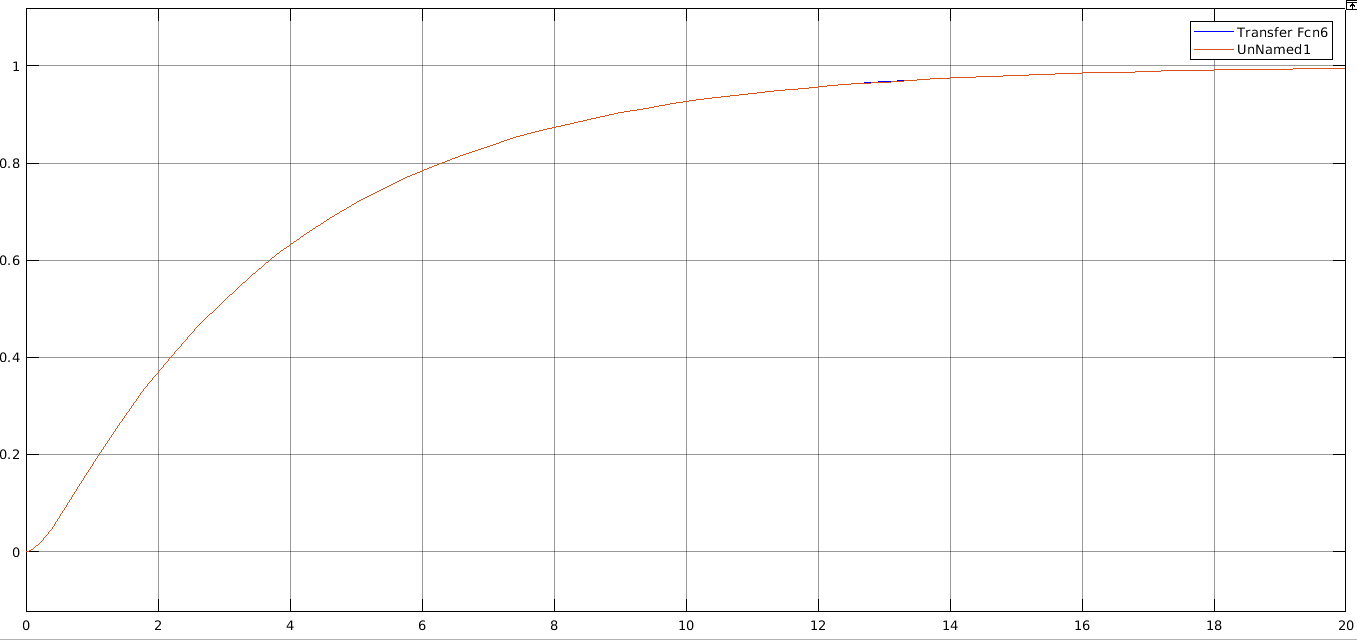
\includegraphics[scale=0.3]{./plot_both1.png}
			\caption{График звена в блоке 1 и передаточной функции}
			\label{fig:pb1}
    	\end{figure}

    \subsection{Блок 2}
		На рисунке~\ref{fig:p2} представлен график звена 2. По его форме можно определить,
		что это колебательное звено.
		$k = 0.25, T = 0.5, \zeta = 0.263$

		Тогда передаточная функция имеет вид (рисунок ~\ref{fig:pb2}):
		\[ W(s) = \dfrac {0.25} {0.25 s^2 + 0.263 s + 1}\]

    	\begin{figure}[ht!]
    		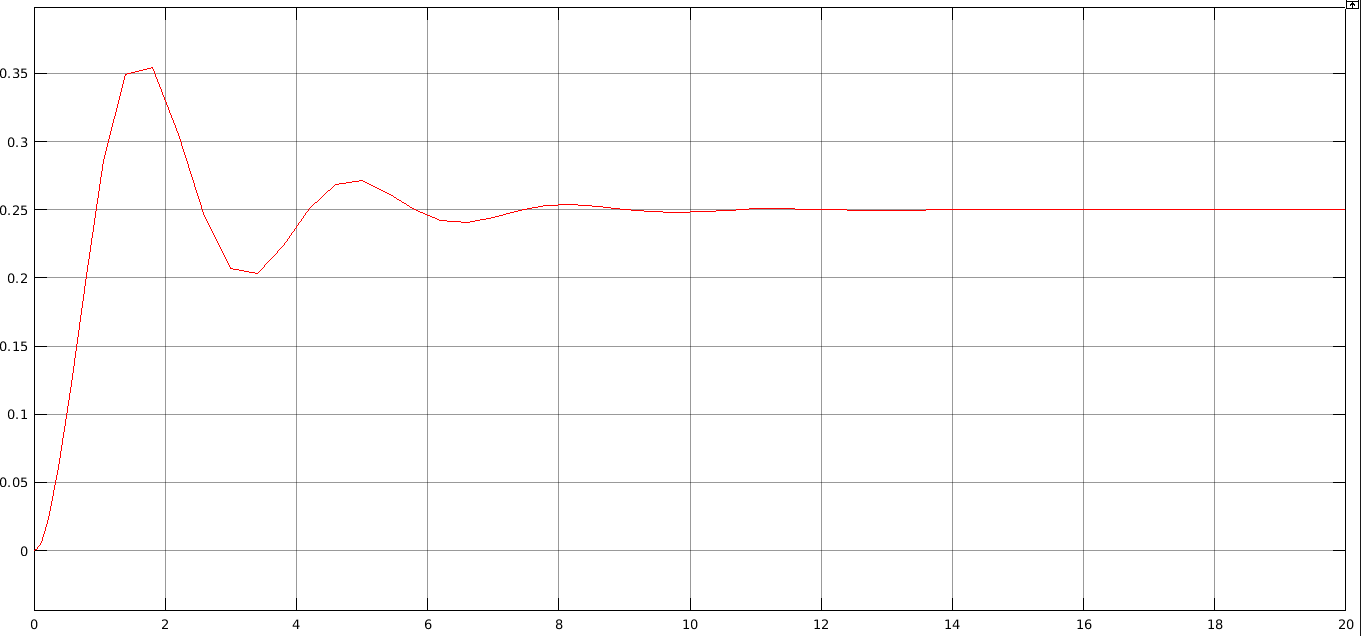
\includegraphics[scale=0.3]{./plot2.png}
			\caption{График звена в блоке 2}
			\label{fig:p2}
    	\end{figure}

    	\begin{figure}[ht!]
    		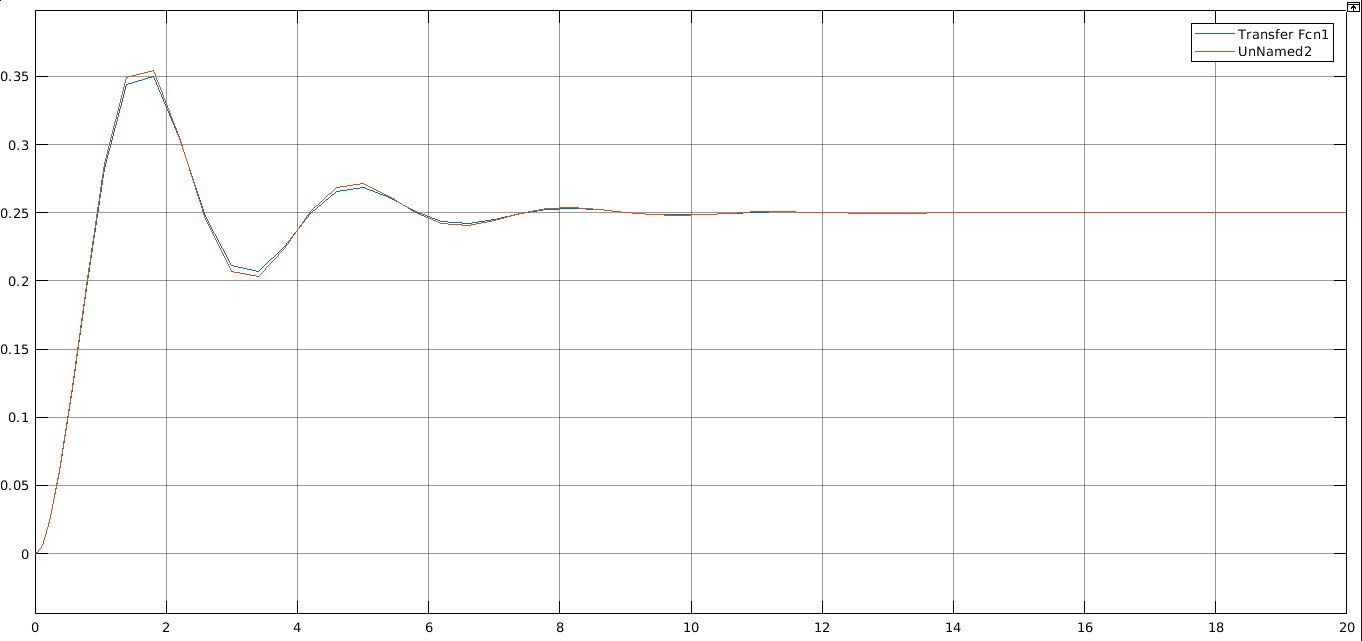
\includegraphics[scale=0.3]{./plot_both2.png}
			\caption{График звена в блоке 2 и передаточной функции}
			\label{fig:pb1}
    	\end{figure}

    \subsection{Блок 3}
		На рисунке~\ref{fig:p3} представлен график звена 3. По его форме можно определить,
		что это апериодическое звено 1-ого порядка: $k = 1, T = 0.2$.
		
		Тогда передаточная функция имеет вид (рисунок~\ref{fig:pb3}):
		\[ W(s) = \dfrac {1} {0.2 s + 1}\]

    	\begin{figure}[ht!]
    		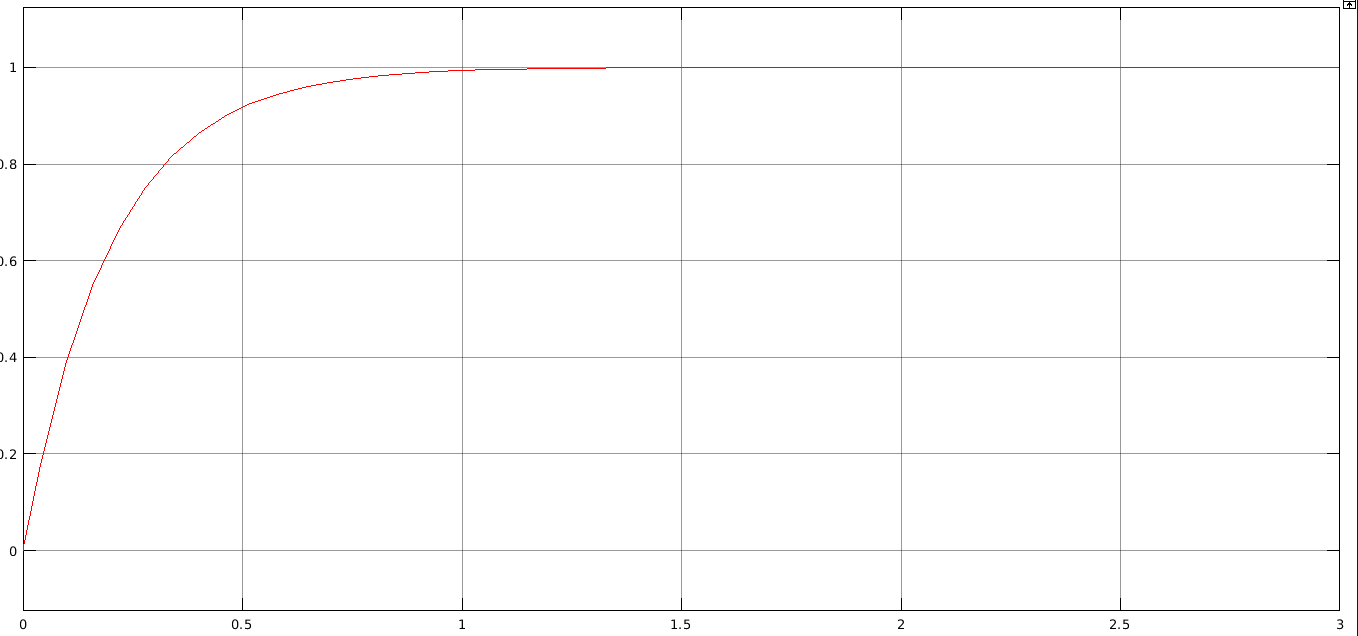
\includegraphics[scale=0.3]{./plot3.png}
			\caption{График звена в блоке 3}
			\label{fig:p3}
    	\end{figure}

    	\begin{figure}[ht!]
    		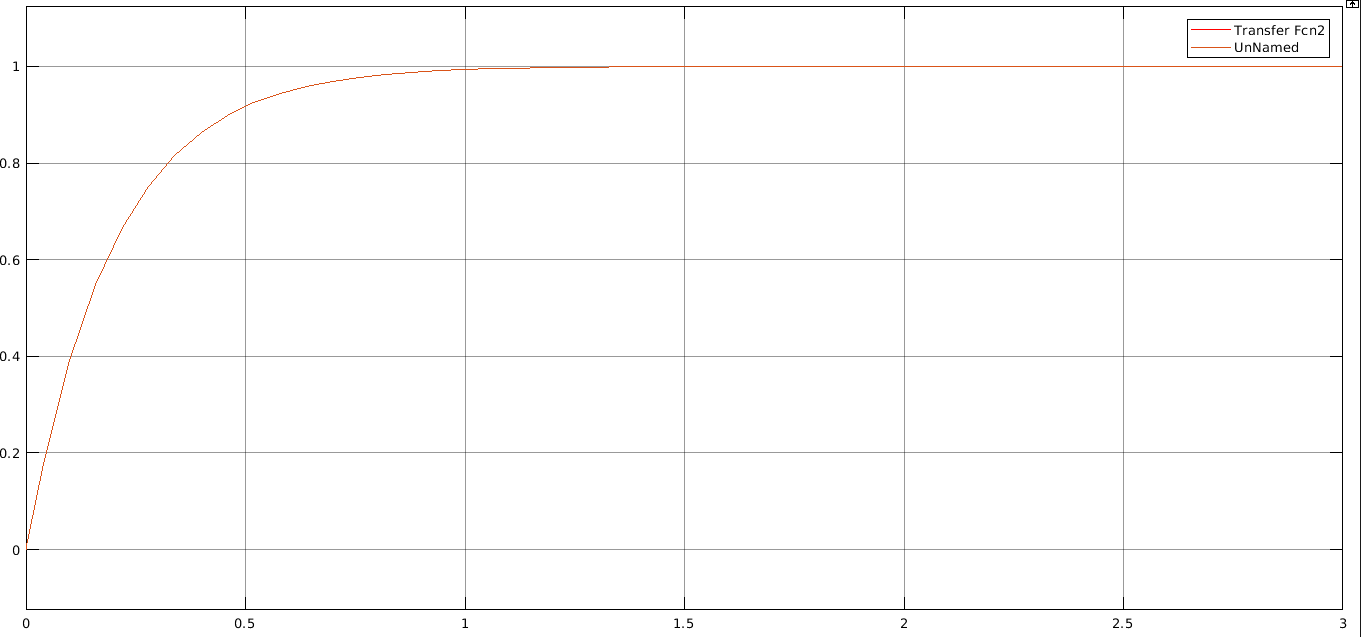
\includegraphics[scale=0.3]{./plot_both3.png}
			\caption{График звена в блоке 3 и передаточной функции}
			\label{fig:pb3}
    	\end{figure}

    \subsection{Блок 4}

		На рисунке~\ref{fig:p4} представлен график звена 4. По его форме можно определить,
		что это интегрирующее звено c замедлением: $k = 2, T = 0.2$.
		
		Тогда передаточная функция имеет вид на рисунке ~\ref{fig:pb4}.
		\[ W(s) = \dfrac {2} {s(0.2 s + 1)}\]

    	\begin{figure}[ht!]
    		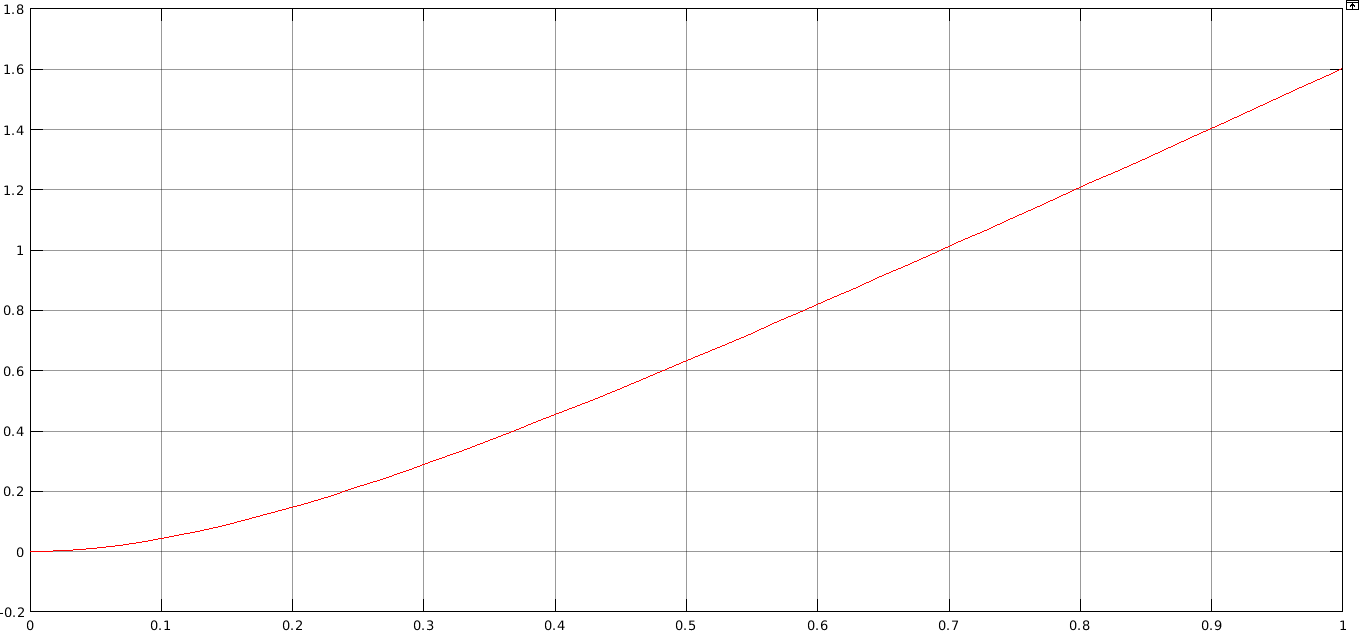
\includegraphics[scale=0.3]{./plot4.png}
			\caption{График звена в блоке 4}
			\label{fig:p3}
    	\end{figure}
    	\begin{figure}[ht!]
    		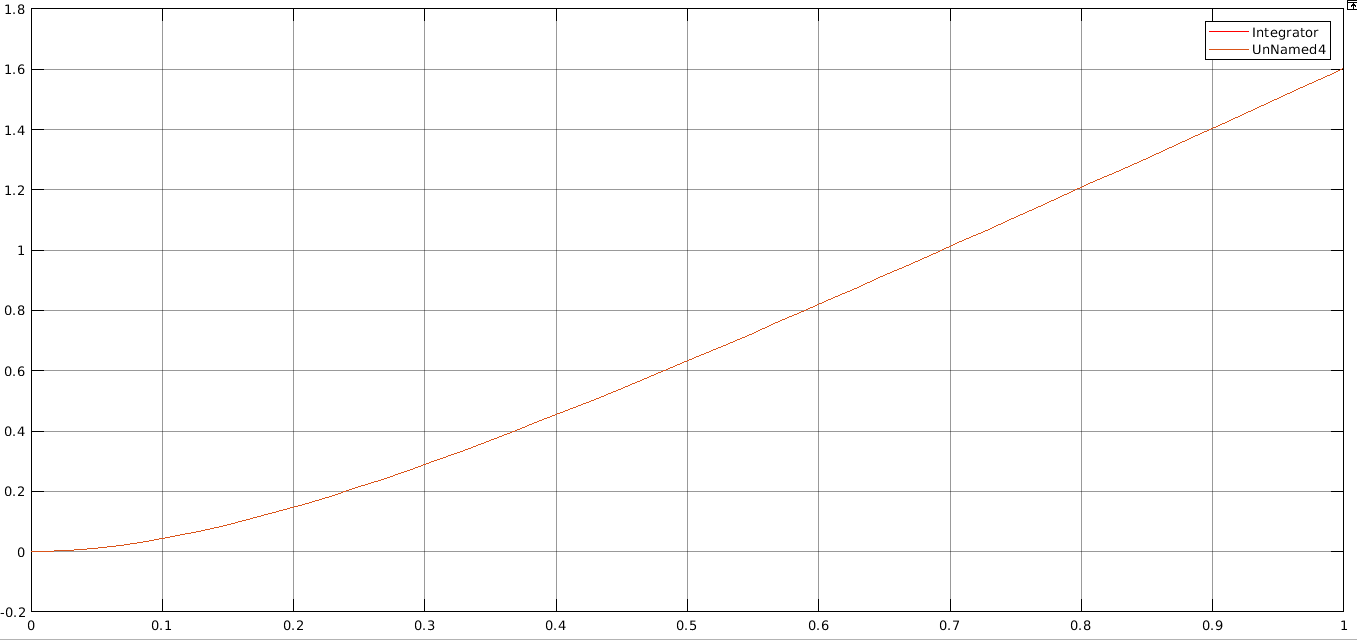
\includegraphics[scale=0.3]{./plot_both4.png}
			\caption{График звена в блоке 4 и передаточной функции}
			\label{fig:pb3}
    	\end{figure}

    \subsection{Блок 5}

		На рисунке~\ref{fig:p5} представлен график звена 5. По его форме можно определить,
		что это реальное дифференцирующее звено: $k = 100, T = 1$.
		
		Тогда передаточная функция имеет вид на рисунке ~\ref{fig:pb5}.

		\[ W(s) = \dfrac {100s} {s + 1}\]

    	\begin{figure}[ht!]
    		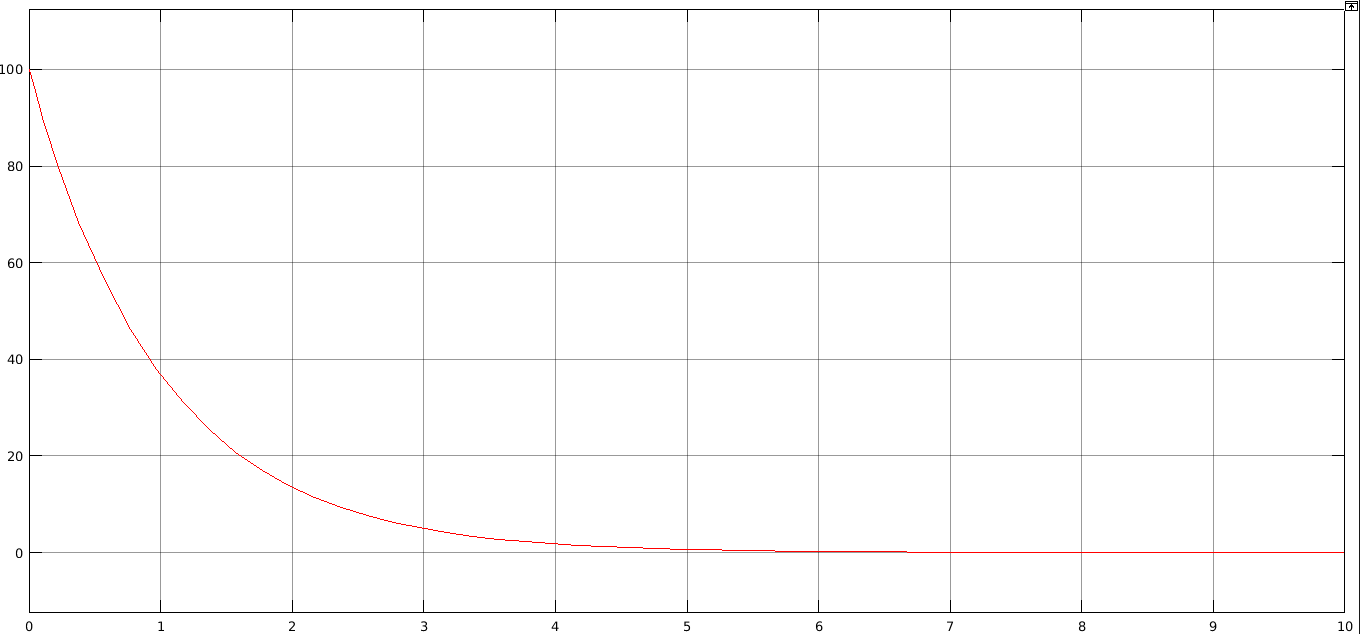
\includegraphics[scale=0.3]{./plot5.png}
			\caption{График звена 5}
			\label{fig:p5}
    	\end{figure}
    	\begin{figure}[ht!]
    		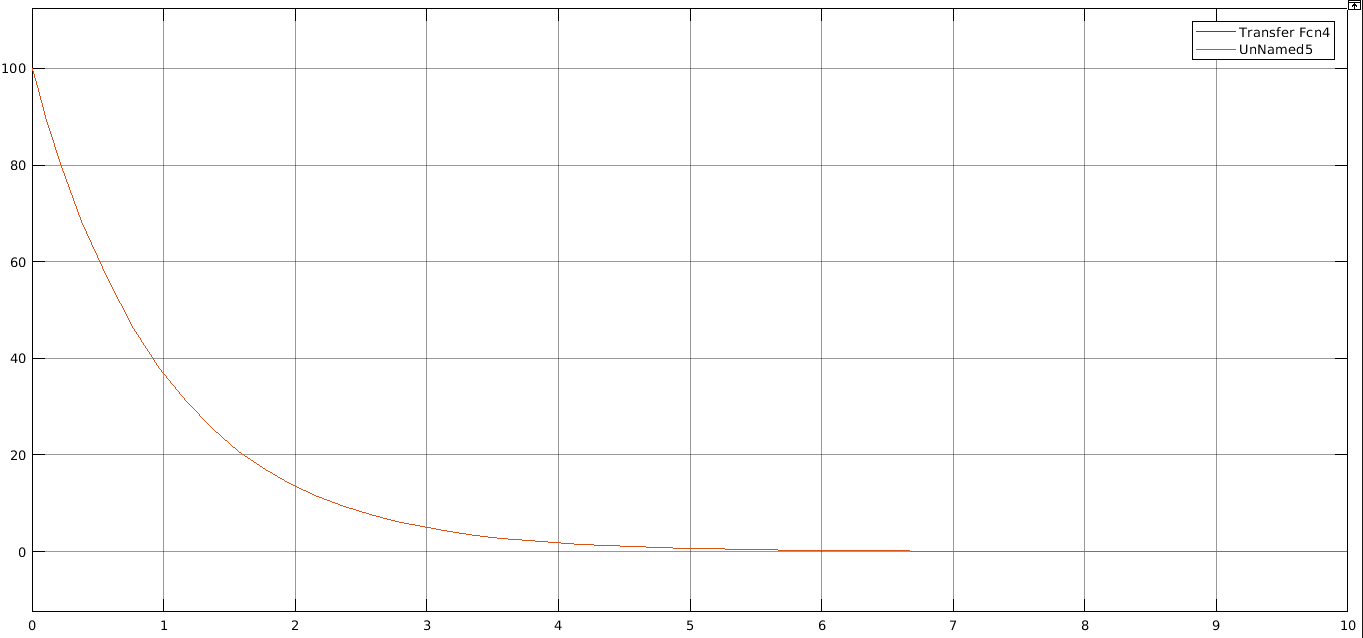
\includegraphics[scale=0.3]{./plot_both5.png}
			\caption{График звена в блоке 3 и передаточной функции}
			\label{fig:pb5}
    	\end{figure}

    \subsection{Блок 6}

		На рисунке~\ref{fig:p6} представлен график звена 6. По его форме можно определить,
		что это интегрирующее звено: $k = 5, T = 1$.
		
		Тогда передаточная функция имеет вид на рисунке ~\ref{fig:pb6}.
		\[ W(s) = \dfrac {5} {s}\]

    	\begin{figure}[ht!]
    		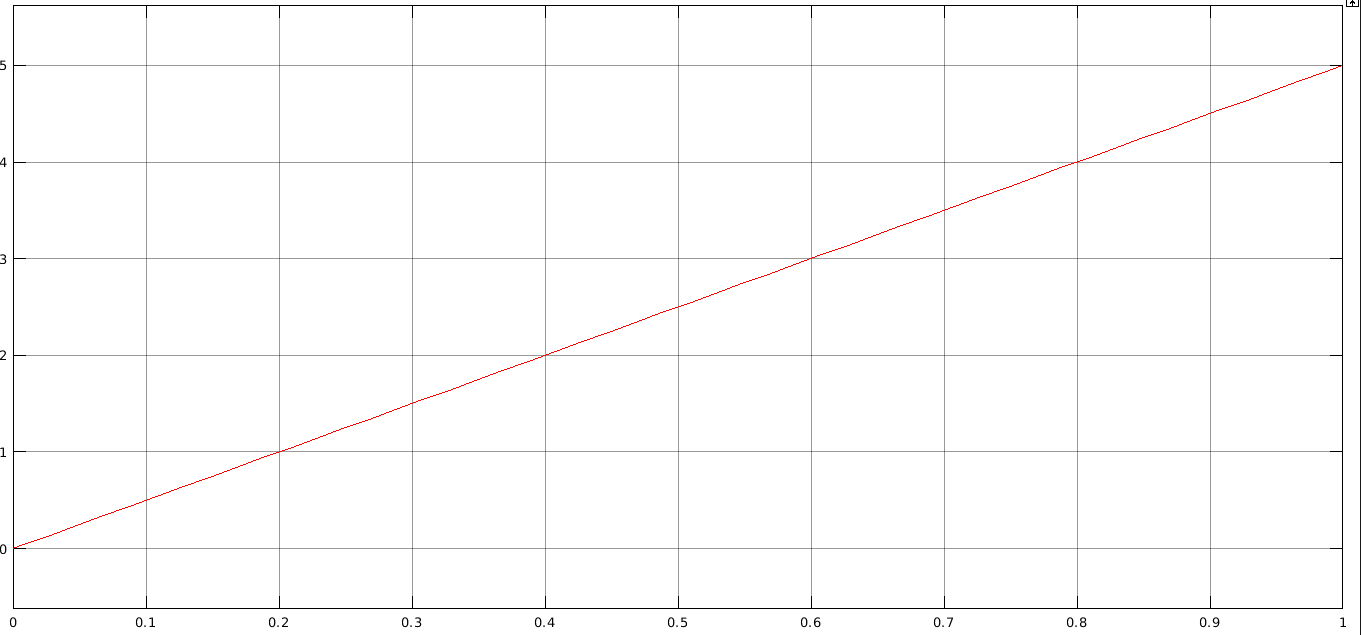
\includegraphics[scale=0.3]{./plot6.png}
			\caption{График звена 6}
			\label{fig:p6}
    	\end{figure}
    	\begin{figure}[ht!]
    		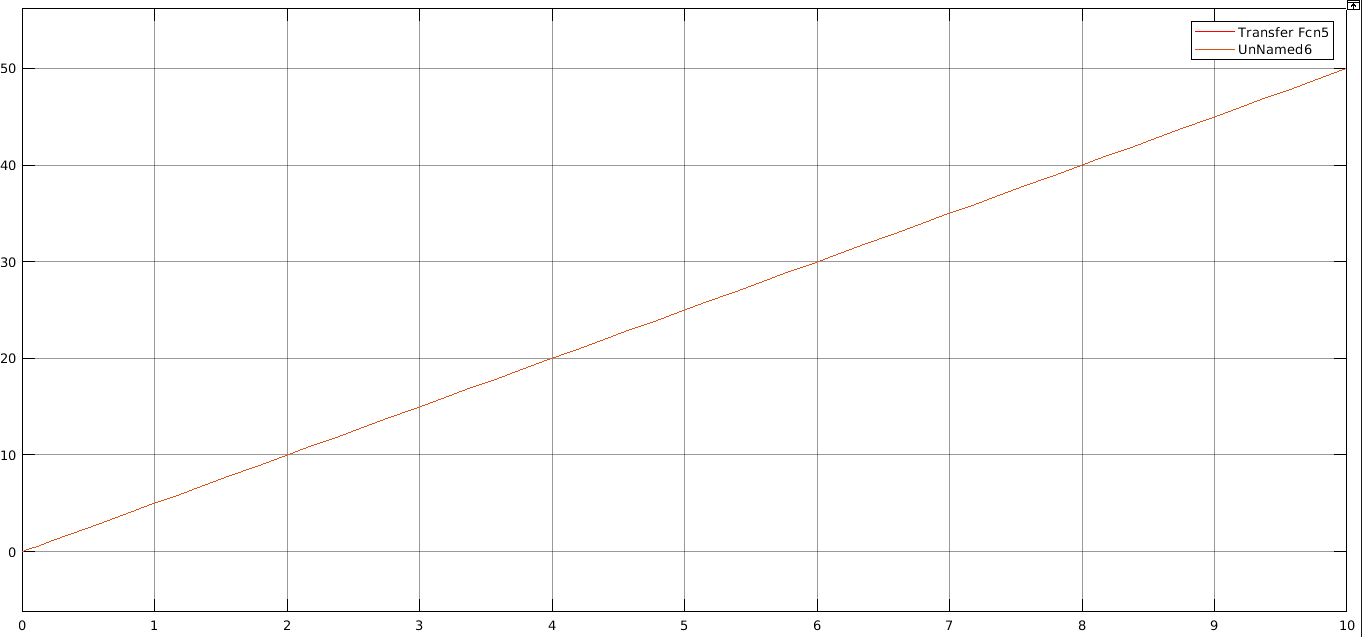
\includegraphics[scale=0.3]{./plot_both6.png}
			\caption{График звена в блоке 6 и передаточной функции}
			\label{fig:pb6}
    	\end{figure}

\section{Вывод}

В ходе выполнения работы было проведено исследование переходных характеристик
элементарных звеньев. При выполнении работы возникли проблемы с выданной
математической моделью, которая не запускалась под имеющейся версией Mathlab,
так что пришлось исправить имеющися скрипт (оказалось достаточно
заменить вызов \\ \texttt{new\_system(subsystem\_name)} на \texttt{add\_block('built-it/SubSystem', subsystem\_name)}
и убрать установление косметических параметров для подсистемы).

\end{document}
